\section{Binary image processing}

\subsection{Binarization}

Goal: Separate foreground and background pixels. Global vs adaptive thresholds.

\subsubsection{Otsu's method}

Minimize threshold of intra-class variance, $p_0 \sigma_0^2 + p_1 \sigma_1^2$,
where $p_i$ is the probability, $\sigma_i^2$ the variance of class $i$.
Equivalent: Maximize inter-class variance $p_0 p_1 (\mu_0 - \mu_1)^2$.

\subsubsection{Niblack's method}

Use local threshold $T_{x, y} = \mu_{x, y} + k \cdot \sigma_{x, y}$, where $k
\in [0, 1]$, typical $k = 0.2$. Window size chosen based on resolution, such
that it contains several characters.

Bad performance if window only includes background!

\subsection{Connected components}

\begin{itemize}
		\item 4-connectivity: Orthogonally connected pixels
		\item 8-connectivity: All neighbouring pixels
		\item n-connected path: Path connected via n-connectivity. E.g.
				4-connected path is akin to movement in Snake, 8-connected path
				akin to movement of queen in chess.
		\item n-connected component IFF for every pair of pixels, there is an
				n-connected path connecting them.
\end{itemize}

\subsection{Jordan's theorem}

In continuous space, a closed simple curve divides the plane into two connected
regions.

In discrete space, a 4-connected curve delimits two 8-connected regions, a
8-connected curve delimits two 4-connected regions.

\subsection{Extracting connected components}

\subsubsection{2D scanning}

Suitable for many small components. Works by only comparing black runs on
current line to those in previous lines. Builds up compoments, merging where
applicable.

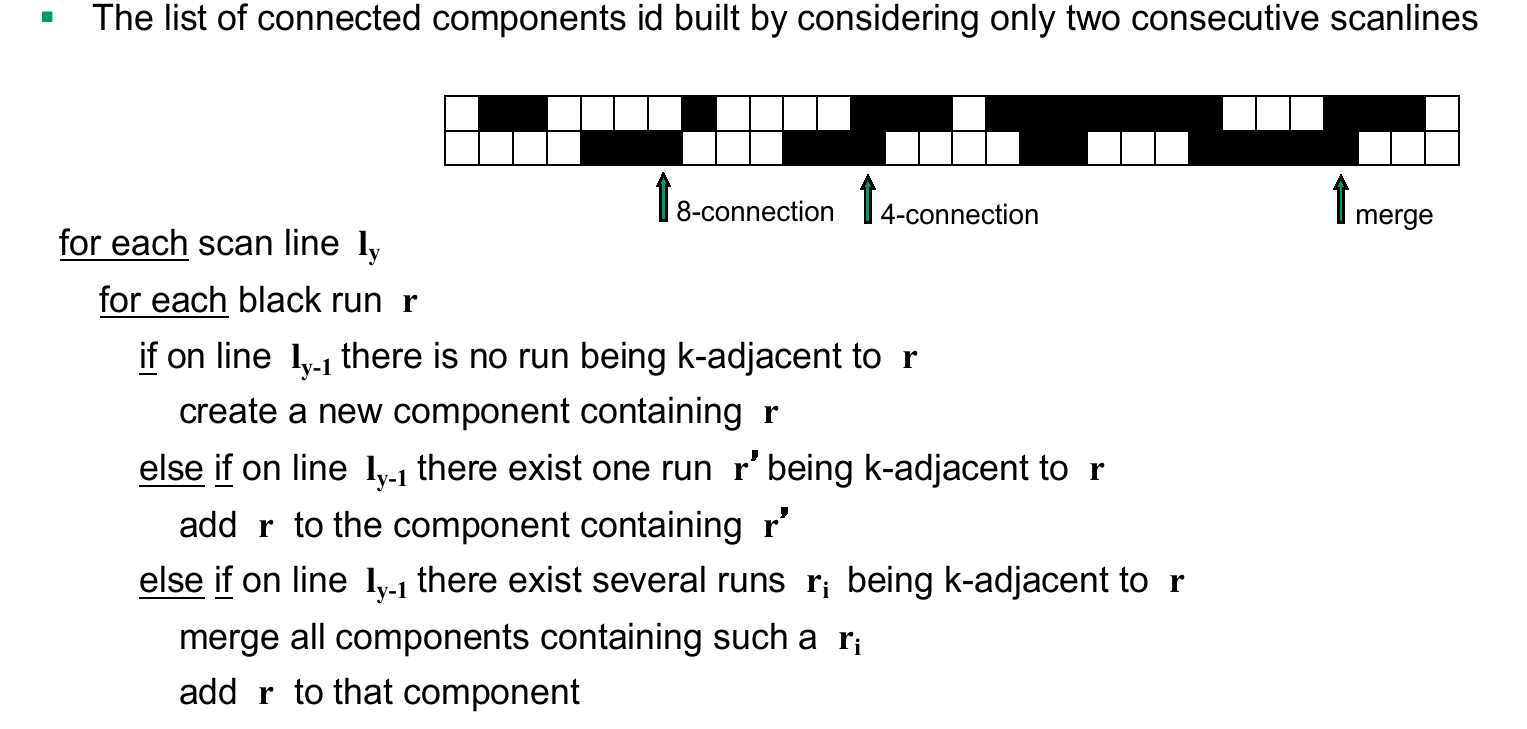
\includegraphics[width=0.5\textwidth]{06_2d_scanning}

\subsubsection{Border following algorithm}

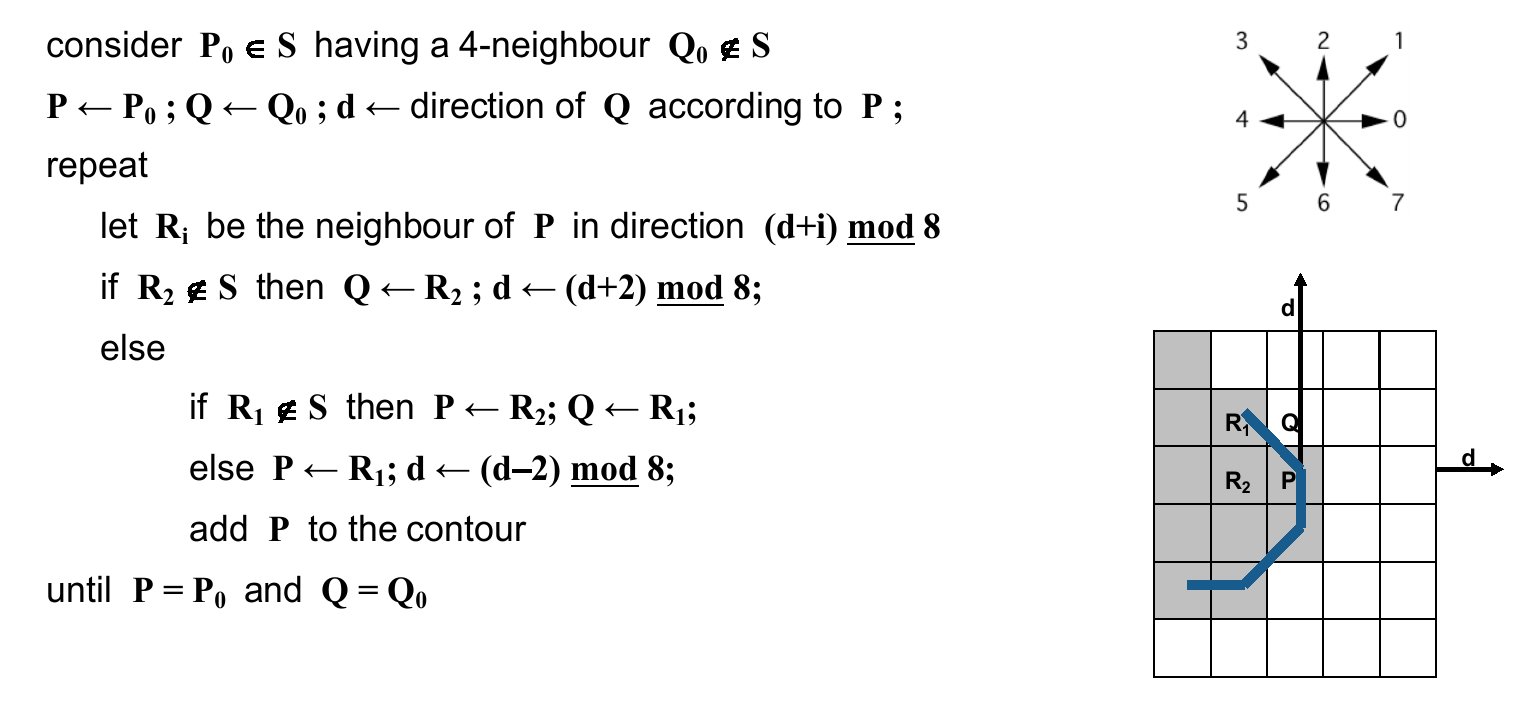
\includegraphics[width=0.5\textwidth]{06_border}

\subsection{Morphological operations}

Operations using a mask (`structurnig element') and an operation, to modify
pixel based on its neighbours. (Local operation).

\subsubsection{Erosion}

Idea: Keep pixels where every pixel of mask has a corresponding pixel on image.
Example mask: Cross shape.

$X \Theta M = \{p | M_p \subset X\}$

\subsubsection{Dilation}

Keep pixels for which any pixel of mask overlaps the shape.

$X \oplus M = \{p | M_p \cap X \neq \emptyset\}$

\subsubsection{Duality of erosion and dilation}

Erosion of inverse is inverse of dilation, and dilation of inverse is inverse
of dilation.

\begin{align*}
		\bar{X} \Theta M = \bar{X \oplus M} \\
		\bar{X} \oplus M = \bar{X \Theta M}
\end{align*}

\subsubsection{Opening and closing}

Let $M^{-}$ be the `symmetric' (mirrored along anchor point) structural
element. If $M$ is symmetric, $M = M^{-}$.

\paragraph{Opening}

Erasion then dilation.

\[
		X \circ M = (X \Theta M) \oplus M^{-}
\]

\paragraph{Closing}

Dilation then erosion.

\[
		X \bullet M = (X \oplus M) \Theta M^{-}
\]

\paragraph{Properties}

\begin{align*}
		\bar{X} \circ M = \bar{X \bullet M}, \bar{X} \bullet M = \bar{X \circ M} && \text{Duality} \\
		X \circ M \subset X, X \subset X \bullet M && \text{Opening is subset, closing is superset of image} \\
		X \subset Y \Rightarrow (X \circ M) \subset (Y \circ M), (X \bullet M) \subset (Y \bullet M) && \text{Monotonically increasing} \\
		(X \circ M) \circ M = X \circ M, (X \bullet M) \bullet M = X \bullet M && \text{Idempotent} \\
		(X \circ M) = \cup \{M_p | M_p \subset X\}
\end{align*}

\subsubsection{Run-length smoothing}

Widely used technique for layout analysis, fill white gaps below a given
threshold horizontally or verticall. Corresponds to opening with $1 \times T$
mask.

\subsubsection{Hit and miss operator}

\[
		\operatorname{ham}_{M_0, M_1}(X) = X \otimes (M_0, M_1) = (X \Theta M_1) \cap (\bar{X} \theta M_0)
\]

Hit and miss operator can be represented as one ternary (three-valued) mask,
where the mask is black where masks one is $1$, white where mask two is $1$,
gray where both masks are white.

\subsubsection{Thinning}

\[
		\operatorname{thin}_M(X) = X - \operatorname{ham}_M(X) = X \cap \bar{(\operatorname{ham}_M(X))}
\]

\subsubsection{Homotopic transformation}

A transformation is homotopic IFF the connexity of all components is preserved,
including wholes. Compare e.g. standard erosion: Can break up components, so is
not homotopic.

Operations can be made homotopic by using special masks.

\subsubsection{Skeleton in euclidean and discrete geometry}

Skeleton $\operatorname{skel}(X)$ of connected component $X$ is all points in
the canters of the maximal inscribed circles. No satisfying of this definition
in discrete space however.

Discrete skeletonization achieved with iterative homotopic transformations,
converting a connected component $X$ into skinny curves.

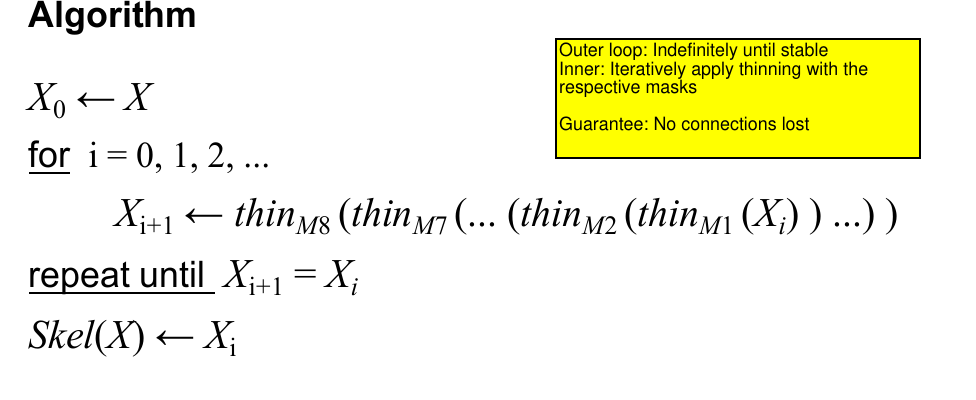
\includegraphics[width=0.5\textwidth]{06_skeletonization}

\subsubsection{Pruning}

Can be used to remove separated pixels after skeletonization. Removes terminal
pixels via hit and miss using certain masks.
